\subsection{Multi-View Network Learning from Multiple Low-Level Visual Clues}
\label{sec:vis2net}

In the previous section, we considered the problem of reconstructing missing links for a multi-view network representation, where we assumed that each type of image features explicitly corresponds to a view in the network representation. In this case, when we extracted for each pair of Facebook users three features describing their mutual relationships, including the number of their shared friends, the number of their co-occurrence in pictures, and their relative poses in images, we may directly reach a three-view network representation $G\triangleq\{A^{(1)}, A^{(2)}, A^{(3)}\}$ (assuming all links are observable). However, this may not be true, when the available types of low-level visual clues are much more than the number of views of interest, and in particular, when the views of the network correspond to higher-level semantics than directly and explicitly related to the low-level visual clues. Let us take the same example used in Section \ref{sec:intro} to illustrate this case.

As shown in Fig. \ref{fig:featurelearn}(a), suppose we have successfully detected two faces $i$ and $j$, and through the state-of-art computer vision techniques we have computed a set of five descriptors characterizing five types of visual clues, including: 1) Relative positions of the two detections (denoted as $\vy^1$); 2) facial expressions (denoted as $\vy^2$); 3) mutual gazex (denoted as $\vy^3$); 4) mutual body poses (denoted as $\vy^4$); and 5) scene classfication (denoted as $\vy^5$). The network we expect to estimate, on the other hand, is a three-view network, where $A^{(1)}, A^{(2)}, A^{(3)}$ both take binary values. $A^{(1)}(i,j)=1$ means the two people belong to the same family and $A^{(1)}(i,j)=0$ means otherwise, $A^{(2)}(i,j)=1$ means the two people are workmates and $A^{(2)}(i,j)=0$ means otherwise, and $A^{(3)}(i,j)=1$ means the two people are friends and $A^{(1)}=0$ means that they do not know each other well. In this example, it is unclear how we may derive the binary socially-characteristic quantities $A$'s from the low-level clues $\vy^1$ to $\vy^5$.


\begin{figure}[t!]
\begin{center}
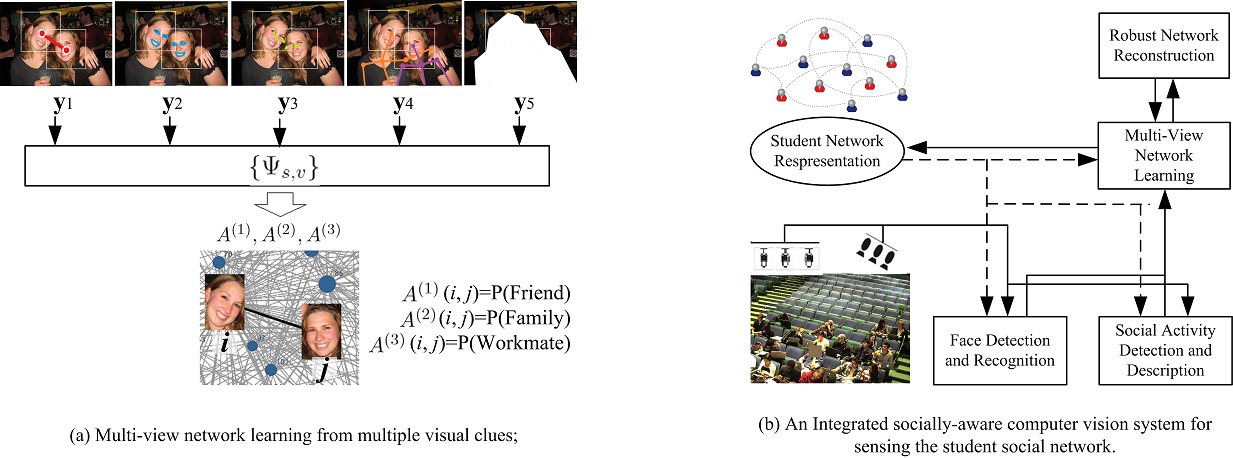
\includegraphics[width=\columnwidth]{featurelearn}
\end{center}
\vspace{-0.25in} \caption{\captionsize 
Illustrations for the problem of multi-view network learning from multiple low-level visual clues and the framework of integrated socially-aware computer vision for understanding student netwrok. \label{fig:featurelearn}\afterfigspace}
\end{figure}


We propose to learn to obtain the high-level multi-view network representations from the low-level visual clues. We refer to this learning architecture as multi-view network learning from multiple low-level visual clues. In general, we assume that there exist $S$ types of low-level `sensors' which provide $S$ types of descriptors $\vy^s, s=1,2,\cdots,S$ that may be relevant to social semantics of the network of $V$ views $A^{(v)}, v=1,2,\cdots,V$. Our architecture consists of $S\times V$ `oracles' $\Psi_{s,v}$, each of which is an estimator $\hat{A}^{(v)}$ of view $v$ from descriptor $\vy^s$, i.e., $\hat{A}^{(v)}=\Psi_{s,v}(\vy^s)$. To learn the optimal `oracles', let us assume that we have $N$ `ground-truth' graphs $G_1, G_2, \cdots, G_N$ associated with their visual clues $\vy^{s}_{n}, s=1,2,\cdots,S, n=1,2,\cdots,N$ computed from related imagery.  Then, the overall learning objective can be represented as 
\begin{equation}\label{eq:sensing}
\{\Psi^{*}_{s,v}\}=\arg\min_{\{\Psi_{s,v}\}}\sum_{n=1}^{N}\mathcal{J}(\{\Psi_{s,v}\}, \{\vy^{s}_n\}, \{A^{(v)}_n\})+\sum_{n=1}^{N}\tau(\{\hat{A}^{(v)}_n\})+\gamma(\{\Psi_{s,v}\}).
 \end{equation}
 
Specifically, we use the first term $\mathcal{J}$ to enforce the estimation quality of the oracles, for example, by defining
\begin{equation}\label{eq:L2error}
\mathcal{J}(\{\Psi_{s,v}\}, \{\vy^{s}_n\}, \{A^{(v)}_n\})=\sum_{s=1}^{S}\sum_{v=1}^{V}\|\Psi_{s,v}(\vy^{s}_n)-A^{(v)}_n\|^{2},
 \end{equation}
such that the estimated network is as close as possible to the `ground-truth' in the sense of minimal $l_2$ error between the affinity matrices. One may image that a conventional regression suffices for this purpose, and powerful regression machines exist, such as support vector regression, Gaussian process regression, as well as deep learning. However, socially-compatible estimations requires more than conventional estimations, in the sense that the individual oracles must give compatible estimates across views. Two nodes inferred as family members by one oracle, for example, should receive low confidence score from the friendship oracle which claims that they are adversary to each other. We use the penalty $\gamma$ to enforce the compatibility among oracles. Finally, we have been fully aware of the community clustering effects of real-world social networks, and therefore we incorporate penalty $\tau$ as well to enforce the clustering effect within the estimated affinity matrix, so that if node $i$ and node $j$ are both inferred as family members of node $k$ we will have the same inference for the relationship between $i$ and $j$. We omit further discussion about $\gamma$ and $\tau$ due to space limitation.


We argue that cross-view compatibility and within-view clustering are essential to any socially-aware `sensors' or computational machines that aim to estimate the social attributes from low-level visual clues, or even other types of conventional clues. This socially-aware sensing architecture, dissimilar to any other regression machines which take in and output independent samples, is at the heart of our proposed research.
